\documentclass[11pt]{article}
%Gummi|065|=)
\title{Homework \#2: Discussion on kNN and Decision Trees\\ for Classifying CNN News Articles}
\author{Doug McGeehan\\
		CS 6001: Applied Spatial and \\ Temporal Data Analysis\\
		Spring 2017}

\usepackage[margin=1in]{geometry}
\usepackage{verbatim}
\usepackage{framed}
\usepackage{amsmath}
\usepackage{amssymb}
\usepackage{graphicx}
\usepackage{caption}
\usepackage{subcaption}

\begin{document}

\maketitle

\section{Experimental Setup}

100 articles from the CNN website were processed into Term Frequency and Tf-idf matrices for this report's experiments.
These articles were selected randomly in such a way as to have an equal portion of articles in each category.
Since there are seven categories present in the CNN article dataset, each category in the subset of 100 articles consisted of 14 to 15 articles.
The results from each experiment were averaged through 5-fold cross validation,
 whereby the dataset was partitioned into five equal-sized subsets, four used for classifier training and one used for classifier testing.
This was repeated five times for all combinations of testing and training partition assignment.
The \texttt{scikit-learn} Python library was used to calculate the precision, recall, and f-scores of each classification task.

\section{Performance of Decision Trees}

The \texttt{DecisionTreeClassifier} of the \texttt{scikit-learn} Python library was used to perform the experiments on Decision Tree supervised classification.
This package creates binary-splitting decision trees using either the Gini index or information entropy gain as the criteria for performing node splits.
Once a decision tree is trained, the 


\begin{figure}[h!] \label{fig:pathlengths}
  \centering
  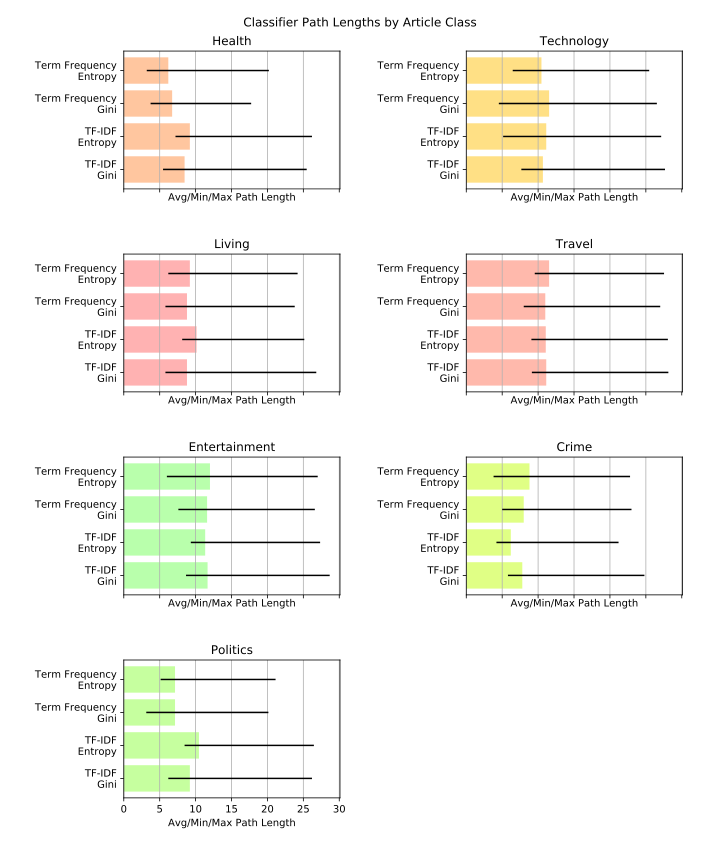
\includegraphics[width=\textwidth]{figures/decision_tree/path_depths}
  \caption{For each article category, the aggregate path lengths overwhich articles traverse is illustrated.
  Each bar corresponds to the average path lengths in a tree, differentiated by how it was constructed: node splitting criterion (entropy or Gini index) and dataset type (term frequency or tf-idf matrices).
  Error bars correspond to corresponding minimum and maximum path lengths.}
\end{figure}


Figure 1 illustrates the average, minimum, and maximum length of the paths through which for an article of a given category traversed to be classified.
From this figure, it is observed that articles from the entertainment, travel, and technology categories required longer paths to perform classifications both on average and at maximum length.
This implies these categories are harder to classify than others.
Beyond those categories, articles from politics, living, and health were the most difficult to classify under entropy trees built from Tf-idf datasets.
Crime articles, on the other hand, were the easier to classify from these trees.
For trees build on Term Frequency datasets, health and political articles were the easiest to classify.

Figures 2a and 2b illustrate the performance metrics obtained using Term Frequency and Tf-idf datasets for training, respectively.
Accuracy, precisions, recalls, and f-scores varied from one criterion-splitting tree to another without a significant overall pattern.

\begin{figure}[h!] \label{fig:perftf_decisiontree}
	\centering
	\begin{subfigure}{.5\textwidth}
	  \centering
	  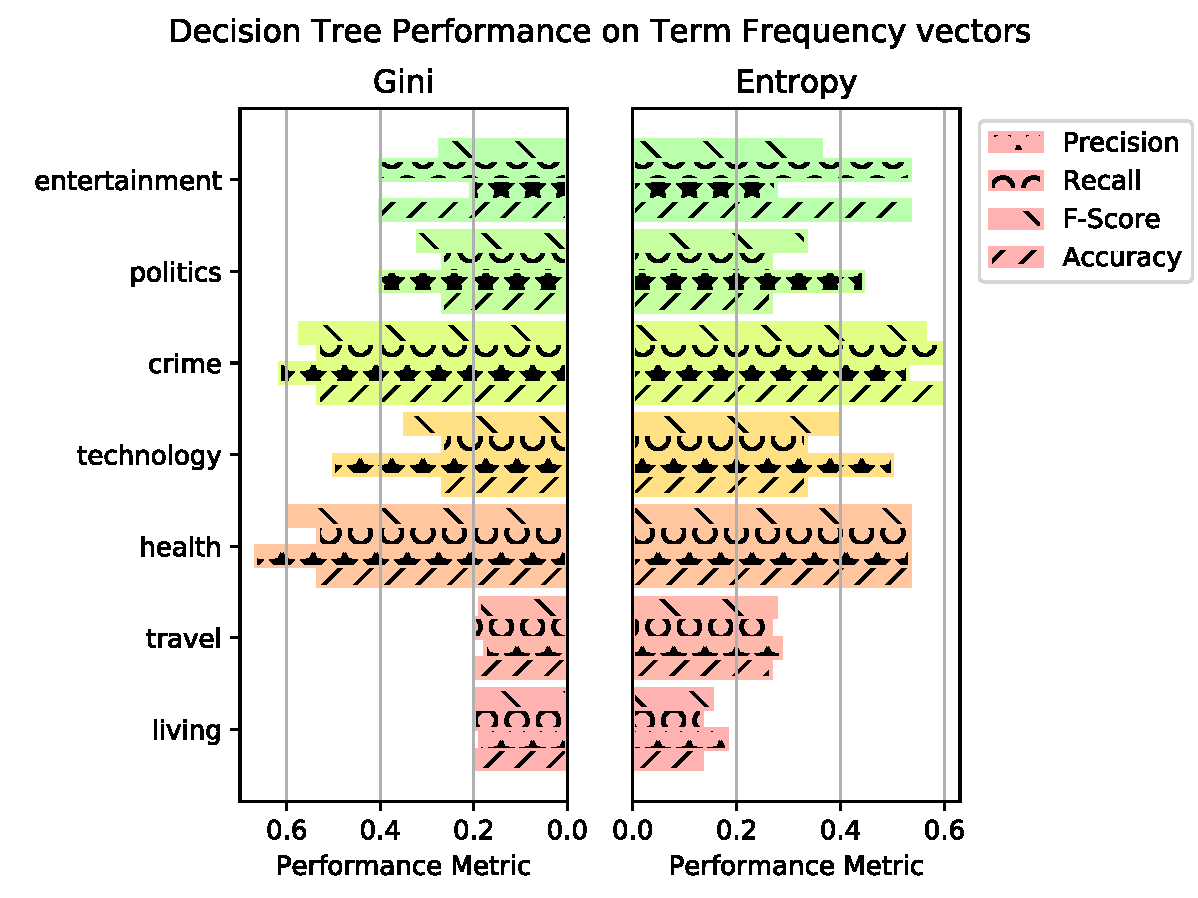
\includegraphics[width=\linewidth]{figures/decision_tree/tf_prec_n_rec}
	  \caption{Performance metrics for Decision Trees trained \\
	  on Term Frequency matrices.}
	  \label{fig:sub1}
	\end{subfigure}%
	\begin{subfigure}{.5\textwidth}
	  \centering
	  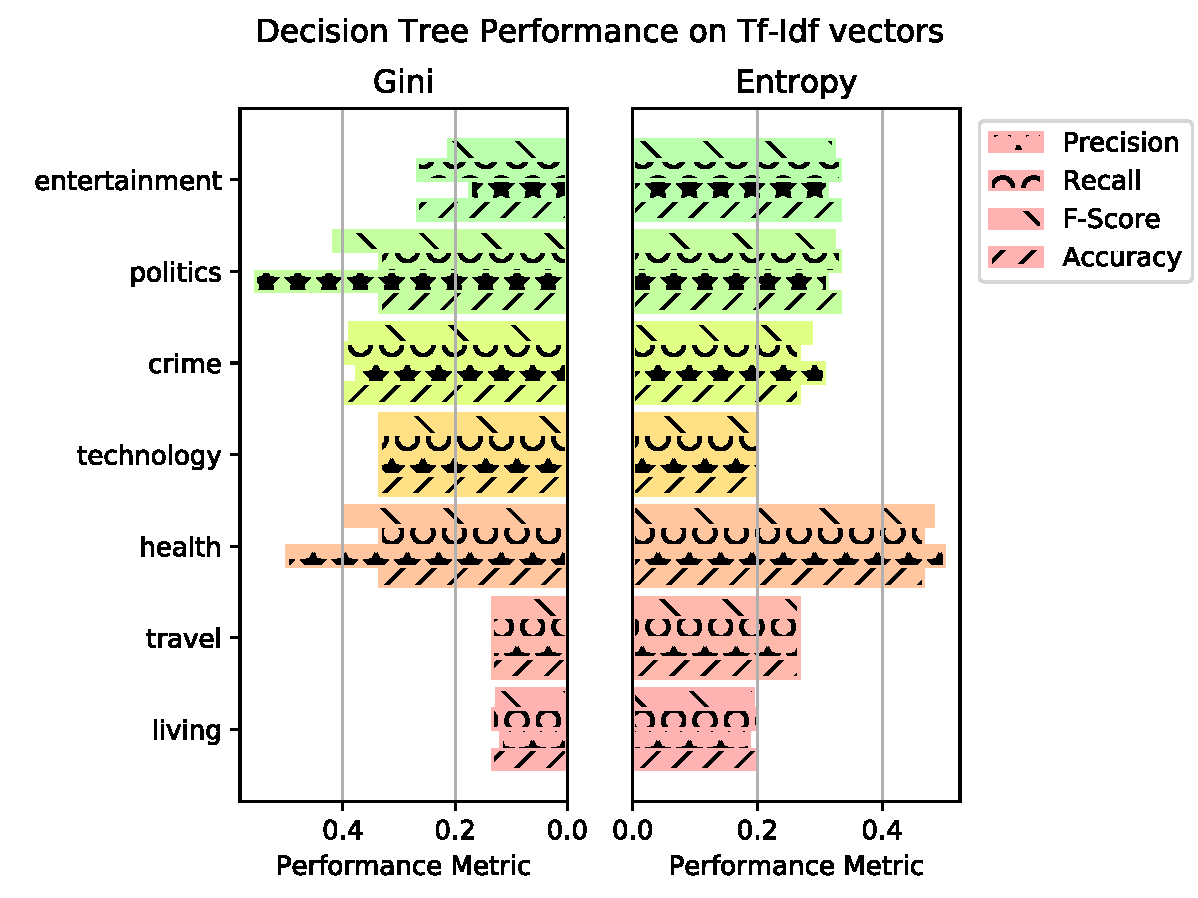
\includegraphics[width=\linewidth]{figures/decision_tree/tfidf_prec_n_rec}
	  \caption{Performance metrics for Decision Trees trained on Tf-idf matrices.}
	  \label{fig:sub2}
	\end{subfigure}
	\caption{A figure with two subfigures}
\end{figure}

For decision trees trained on Term Frequency datasets, accuracies in classification were moderate to low. Health and crime articles were relatively more accurately classified than other article categories by achieving accuracies above 50\%, with crime articles resulting in the highest accuracy of $\approx$60\% on entropy-split trees.
Travel and living articles, however, were classified at the poorest rate, with performance not exceeding 20\% on all metrics (with the exception of travel articles on an entropy-split tree gaining $\approx$30\%).
It should be noted that articles from the living category were successsfully classified by an entropy-splitting tree with approximately the same results as random classification.
Its accuracy, precision, and recall did not exceed 17\%.

Decision trees trained on Tf-idf datasets performed slightly lower than those trained on Term Frequency datasets.
Across all article categories, accuracy and recall did not exceed 50\%.
Of these categories, politics achieved the highest precision at 58\% under Gini-splitting trees, and health articles obtained an accuracy and recall of $\approx$50\% and a precision of $\approx$57\%.
With the exception of health articles under an entropy-splitting tree, recalls did not exceed 40\%.
Finally, travel and living articles were classified with the worst performance overall, with those on a Gini-splitting tree performing worse than random guessing.

\section{Discussion on k-NN Classification}


\bibliography{bibliography}{}
\bibliographystyle{plain}
\end{document}
